%
% $Id: ch01_overview
%
%   *******************************************************************
%   * SEE THE MAIN FILE "AllegThesis.tex" FOR MORE INFORMATION.       *
%   *******************************************************************

\chapter{Introduction}\label{ch:intro} % we can refer to chapter by the label

%   ************************************************************************
%   * In LaTeX, new paragraphs are begun by simply leaving a blank line in *
%   * the LaTeX file.                                                      *
%   *                                                                      *
%   * The \\ characters should NEVER be used to end a paragraph.           *
%   * They are used only for inserting line breaks in certain situations.  *
%   *                                                                      *
%   * "Widows" (ending paragraph lines at the top of a new page) and       *
%   * "orphans" (opening paragraph lines at the bottom of a page) should   *
%   * be eliminated; this sometimes requires re-writing some of the        *
%   * text to change the line lengths.                                     *
%   ************************************************************************

Our research focuses on the development of intelligent agents for playing perfect information games.  Specifically, we implement agents for playing the game Go, Hex, and Sprouts, which we will thoroughly describe later.  The purpose of this chapter is to outline our motivation behind researching this problem, state the goals of our research, and introduce Monte-Carlo Tree Search (MCTS), an algorithm which is very often used for game-playing agents.  We also explain the rules of Go, Hex, and Sprouts, as well as common structures found within the games.

\section{Motivation} \label{sec:motivation}
A major long-term goal of artificial intelligence research is to create a general intelligent agent --- a machine which can act independently, and intelligently, in a variety of situations.  In other words, create a machine which is able to mimic human intelligence.  AI systems already excel in some areas.  For example, in recent years, research into deep neural networks has led to systems which perform very well at pattern recognition problems \cite{imagenet}.  Using a large amount of training data, they are able to perform tasks such as label objects in images\cite{imagenet}, interpret human speech\cite{HintonDeng}, distinguish faces from one another\cite{parkhi15}, and even mimic human speech\cite{wavenet}.  Essentially, such systems can learn to mimic human senses and classification abilities.

However, human intelligence is far more than recognizing patterns and understanding the things we sense.  The ability to react to our world, solve problems, and adapt to changes is much more important when defining true intelligence.  Therefore, in order to progress towards the goal of a more generalized AI, we need to build systems which exist in and adapt to changing environments.

One's first instinct in developing general AI may be to use physical robots as intelligent agents and the real world as an environment.  Robots have been (and continue to be) used in AI research and competitions --- for example, the RoboCup Soccer \cite{robocup} tournament is an annual competition which pits cooperative multi-agent robot systems against one another in games of soccer (Figure \ref{fig:robocup}).  The teams of robots consistently improve every year.  Despite this, their limitations are very obvious.  A quick google search yields many results of the robots failing to do what they were designed to.

\begin{figure}[h]
    \centering
    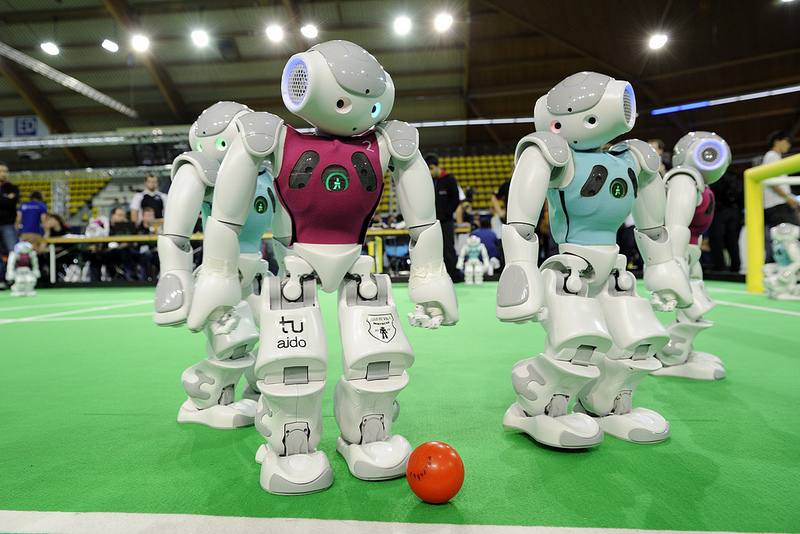
\includegraphics[clip, scale=.25]{images/robocup2015.jpg}
    \caption{RoboCup 2015 \cite{robocup}}
    \label{fig:robocup}
\end{figure}

This is an example of why robots are not ideal for developing AI algorithms --- robots are expensive to build, time-consuming to test, and their effectiveness is bottlenecked by their physical limitations \cite{Gunderson}\cite{Bihlmaier}; they are not an effective way to test algorithms.  Furthermore, there are many variables of the real world which we are simply unable to control effectively, e.g. gravity.  Robots do hold a very important place in the field of AI and computer science in general, but they are not suited for testing new and improving algorithms.  Purely virtual environments --- specifically computer board games --- though, are perfect for experimentation for several reasons.

When working with software agents rather than robots, we do not need to worry about the physical efficacy and limitations of the agents --- the integration of hardware and software is not needed.  Meanwhile, the board game has a set of rules which cannot be broken, and a very obvious goal for everyone in the game: to win.  Furthermore, the rules and win-conditions can be tweaked as needed, and the game can be sped up to allow for quick learning and testing.  Simply put, such games offer extremely controllable environments.  The clear goal (to win) allows for very easy experimentation and testing of game playing agents.  To see how an agent compares against humans, we can simply have the AI play a number of humans to see how often it wins.  We can also have two different agents compete head to head against one another.

Perfect information games are a subset of games for which each player has access to all of the game information --- nothing is hidden from either player.  For example, chess and go are both perfect information board games as both players know the location of any and all pieces on the board.  However most card games, or a game such as Stratego, are imperfect information as the value of each players pieces are hidden from one another \cite{Policonomics}.

When comparing two agents in a head to head game, we consider perfect information to be superior to imperfect information games.  This is because perfect information ensures that the reason for an agent's win is actually a superior algorithm.  In an imperfect information game, there could be pieces of information which are more valuable than other pieces of information --- results of the game could be skewed towards whichever AI stumbles upon this information first \cite{Gilpin}.  For example, in Stratego, the value of a player's piece is hidden from their opponent until an "attack" is made against the piece --- if one player happens to find higher level pieces than their opponent early in the game, the game may become skewed in their favor through pure luck.  While it may be possible to account for such situations (or such imbalances may begin to even out over many trials), it can be easier to just begin with a perfect information game.

In any intelligent game-playing agent, the most important factor is the ability of the agent to evaluate the game state --- that is, the methodology it uses to determine the probability of winning the game for a given state.  For this, one might consider building a system which attempts to identify patterns among positive game states and construct a set of beliefs to approximate the value of any given state; this set of beliefs can be thought of as an evaluation function or heuristic.  However, building an adequate evaluation function for a game state is a very complex task; in fact, there has been much research into using heuristic analysis with little success \cite{chaslot2008monte}.

Tree search methods are another way of determining the value of a game state.  A tree search method simulates a number of full games from the given state, attempting to fully construct a tree of all possible game configurations from the current state --- this tree is called the game tree.  Rather than trying to directly analyze the value of a given game state, a tree search method determines value of a game state by finding how many paths to a winning position exist.

As a tree search algorithm runs, the game tree becomes fuller; once the tree is full, an agent utilizing it is able to play perfectly --- that is it will always win provided it is possible.  The downside of many tree search algorithms is that they are not useful until the game tree is at least mostly full.  In the minimax algorithm, for example, a node's value cannot be determined until the value of every one of its children down to the leaf nodes is found.  For a game such as Go, this is impossible to achieve in any reasonable amount of time --- a single game of traditional 19x19 Go has over $2 \times 10^{170}$ possible playouts.  The exact number of possible Go games was only recently calculated, and required an estimated 30 petabytes of disk I/O \cite{Trompfinal}.  Note this isn't actually constructing the game tree, just calculating how large it would be --- it is actually theoretically impossible to even come close to constructing the whole game tree with today's computing capabilities, due to the sheer amount of storage needed to keep track of everything.

Over the last decade, game AI development has moved away from basic tree search and towards methods involving the Monte-Carlo Tree Search (MCTS) algorithm.  MCTS asymmetrically explores the game tree by taking into account both the current estimated value of each child node, and the number of times each child node has been visited in a simulation.  The specific method of exploration can be customized by considering one of these factors more heavily than the other.  MCTS is also different from other tree search algorithms as it does not need to construct an entire game tree in order to make a decision.  Such methods have proven far more successful, as MCTS-based AIs have since become some of the most successful game AIs in the world \cite{alphago}\cite{benzene}.
%   *******************************************************************
%   * FIGURES ARE PLACED ACCORDING TO A SET OF CONSTRAINTS THAT CAN   *
%   * BE MANIPULATED TO SOME DEGREE.                                  *
%   * A SEARCH FOR "controlling latex floats" TURNS UP A NUMBER OF    *
%   * SITES THAT HAVE USEFUL INFORMATION, FOR EXAMPLE:                *
%   *                                                                 *
%   * http://mintaka.sdsu.edu/GF/bibliog/latex/floats.html            *
%   * http://goo.gl/aC8E8Q                                            *
%   * http://robjhyndman.com/hyndsight/latex-floats/                  *
%   *******************************************************************

\section{Monte-Carlo Tree Search}\label{sec:stateofart}
Monte-Carlo Tree Search (MCTS) is a selective search method for finding optimal decisions via random sampling. Since its development in 2006, it has been widely used for the creation of game AI, specifically for games which can be represented as a finite tree of moves \cite{browne2012survey}\cite{chaslot2008monte}.

MCTS is superior to other popular tree search methods such as minimax for a couple of reasons.  First, while an agent utilizing minimax guarantees optimal play, minimax requires the entire game tree be explored --- this often requires an impractical amount of time for games with even just a moderate branching factor.  MCTS, however, can be interrupted at any time and return a node to explore.  Second, given adequate time, MCTS provides optimal play given adequate memory and time --- in fact, MCTS converges to minimax \cite{browne2012survey}.  So essentially, MCTS can provide accurate decision making without the potentially exponential time complexity of minimax.  

MCTS works in four steps as depicted in Figure 2: Selection; Expansion; Simulation; and Backpropogation.
\begin{enumerate}
    \item  Selection: Starting at the root of the tree, child nodes are selected recursively until a leaf node $L$ is reached.  The way in which these children nodes are selected is called the \textit{tree policy}, and is discussed below.
    
    \item Expansion: if $L$ is not a terminal node for the game tree, a child node $C$ is created.  Depending on the application of MCTS, more than one child node may be chosen.
    
    \item Simulation: Simulate a full play of the game from node $C$.  In the simulation step, the tree policy is not used during the simulation.  Rather, a \textit{default policy} is used --- most commonly, the default policy is a simple random selection from possible moves until a terminal condition is met.  Note that the nodes visited during simulation are not added to the tree.
    
    \item Backpropogation: The tree is updated with the results of the simulation.  Specifically, each node's estimated value is updated (based on the outcome of the simulation), as well as the number of times it has been visited.
\end{enumerate}

\begin{figure}[h]
    \centering
    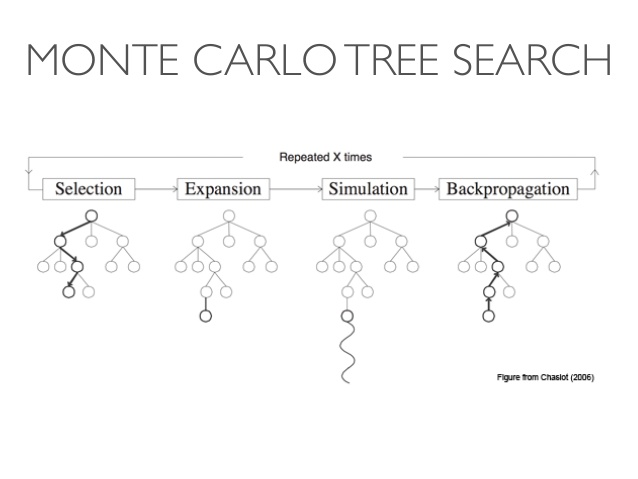
\includegraphics[clip, trim={0 4cm 0 5cm}, scale=.6]{images/mcts.jpg}
    \caption{Monte-Carlo Tree Search algorithm \cite{chaslot2008monte}}
    \label{fig:MCTS}
\end{figure}

During the selection phase, there is a trade-off between \textit{exploitation} and \textit{exploration} --- should we \textit{exploit} the nodes whose rewards we already know, and continue to expand a well searched path, or should we \textit{explore} the less visited nodes in hopes of finding a better option \cite{nakhost2009monte}?  A widely used tree policy to balance these options is called Upper Confidence Bounds for Trees (UCT).  When using UCT as the tree policy, a child node which maximizes the following is chosen:
    
\begin{equation}
    UCT = v_i + C * \sqrt{\frac{2\ln N}{n_i}}
\end{equation}
    
where $v_i$ is the estimated value of the node, $n_i$ is the number of the times the node has been visited and $N$ is the total number of times that its parent has been visited.  $C$ is a constant bias parameter which we can change as we wish.  In this formula, $v_i$ represents exploitation, while the rest of the equation represents exploration.  So, by properly tuning the value of $C$, we are able to find a balance between exploitation and exploration \cite{lucas2014fast}\cite{audibert2009exploration}.

While MCTS can be rather effective in its most basic form, it is further enhanced using a variety of machine learning techniques.  Most of the industry leading game-playing agents utilize an MCTS decision making algorithm with the integration of some other AI techniques --- most often, some form of Artificial Neural Network (ANN) or Genetic Algorithm (GA) is used.  These algorithms and existing implementations of game-playing agents which utilize these algorithms will be discussed in Chapter 2.

%It is the privilege of the thesis author (in consultation with the
%project supervisor and other readers) to decide on the best way to 
%organize the sections and chapters in the way that makes the most sense.
%If the introduction begins with a motivating
%anecdote, perhaps this is best followed by defining a few terms or mentioning
%some major results that the reader should be aware of right from the 
%beginning. But 

\section{Games}\label{sec:goals}
In this brief section, we outline the perfect information games we use for our experiments: Go, Hex, and Sprouts.  Go and Hex are two rather well-known and studied games, while Sprouts has been less popular in research.  The purpose of this short section is to give the reader an understanding of how the games are played.

\subsection{Go}
Go is a two-player game usually played on a 19x19 board, although boards of size 9x9, 13x13, and 17x17 are also common.  The rules of Go are very simple.  The players take turns placing stones on the board, attempting to surround more territory than the other player.  Stones cannot be removed, but if one or more of a player's stones are completely surrounded by the other's, the surrounded stones are removed from the board (Figure \ref{ref:gogui}).  The game continues until either neither player wishes to move or one player resigns.

\begin{figure}[h]
\centering
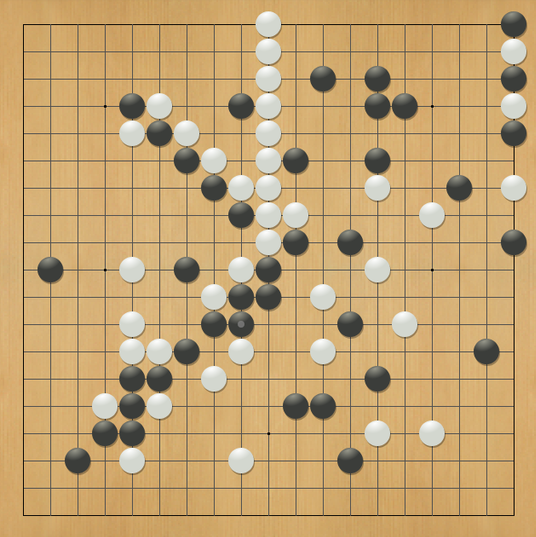
\includegraphics[scale=0.25]{images/gogui.png}
\caption{A Go board generated in GoGui}
\label{ref:gogui}
\end{figure}

Despite its simple rules, Go has over $2 \times 10^{170}$ possible playouts, making it one of the most computationally complex board games ever created \cite{Trompfinal}.  The combination of this fact with its popularity as a game has led to it being the focus of a large amount of research, compared to other games.

\subsection{Hex}
Hex is a two-player board game usually played on a hexagonal grid, usually a 14x14 rhombus as shown in Figure \ref{ref:hex}.  Each player takes turns placing a stone on a cell of the grid, and simply attempts to link their two opposing sides before the opponent links the other two.  The first player to connect their two sides wins.  The only other rule is that, due to the first player to move having a distinct advantage, the second player can choose to switch positions with the first player after the first move.

\begin{figure}[h]
\centering
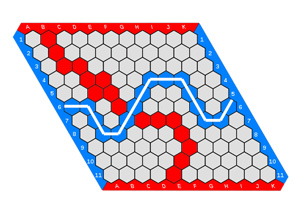
\includegraphics[scale=0.4]{images/hex.jpg}
\caption{A winning game for blue \cite{hexwiki}}
\label{ref:hex}
\end{figure}

\subsection{Sprouts}
Sprouts is a two person pencil-and-paper game which was created by John Conway and Micheal Paterson at Cambridge University in the 1960s. The game has two players, and begins with any number of dots on a piece of paper. The two players take turns drawing a line either between two dots or from one dot to itself. When this line is drawn, a new dot is placed on the line splitting it in half. The last player who is able to legally draw a line wins. A line is only legal if it does not cross any other lines. Furthermore, no vertex can have more than 3 lines coming out of it --- a play on a vertex which already has 3 lines is illegal. The game ends when no moves are possible, and the last player to make a legal move wins.

\begin{figure}[h]
\centering
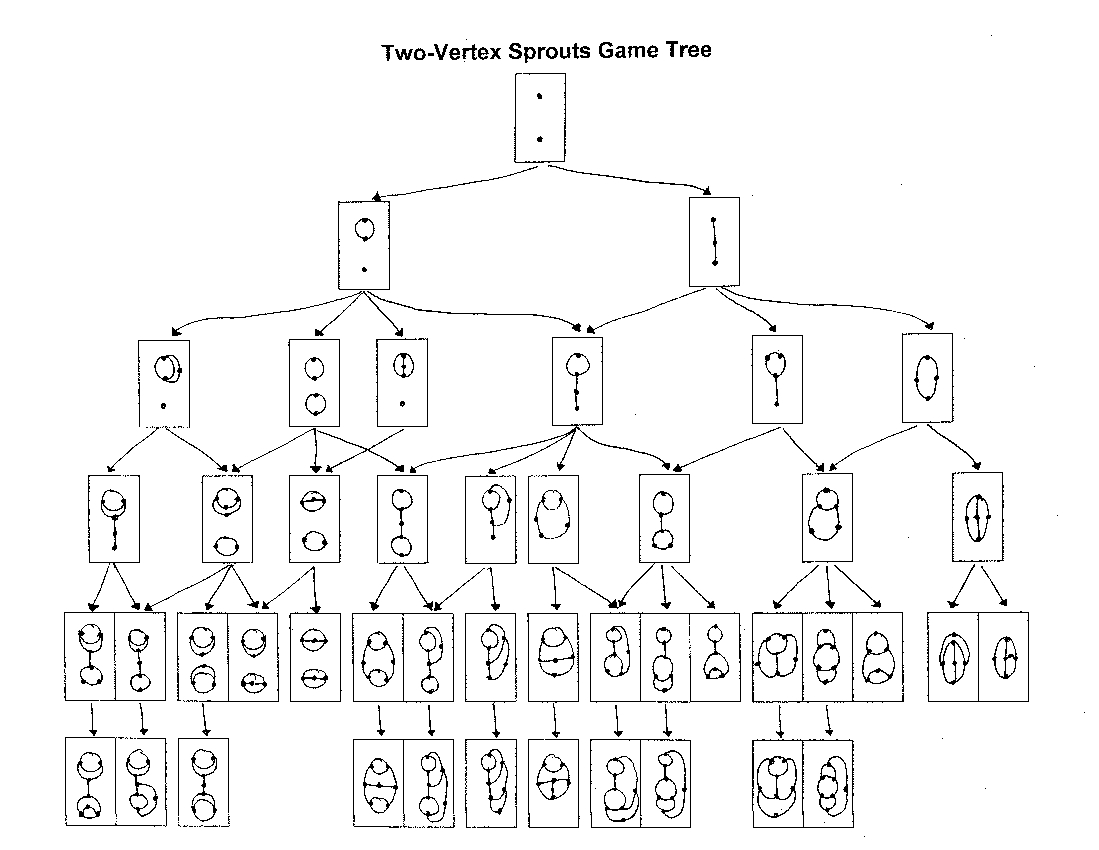
\includegraphics[scale=0.5]{images/sproutsgametree.jpg}
\caption{2 vertex game tree for Sprouts \cite{sproutstree}}
\label{ref:sprouts}
\end{figure}

Figure \ref{ref:sprouts} shows the game tree for the simplest possible game of sprouts --- one with only two starting vertices. As new vertices are added to the start of the game, the tree grows very rapidly.  Because of the simplicity of games with a small number of starting nodes, Sprouts has been completely solved for up to 32 starting vertices --- that is, if the number of starting nodes is at most 32, one can play a perfect game and force a win depending on whether they move first or second \cite{lemoine}.

\section{Goals of the Project}\label{sec:goals}
As stated previously, most of the best current game-playing agents utilize MCTS with some integration of another AI algorithm.  These agents are almost always shown to perform better than agents using just MCTS or other decision making algorithms.  However, they have rarely if ever been directly compared to one another.  This thesis helps fill this gap in research.  We implement a number of intelligent game-playing agents using MCTS integrated with machine learning algorithms which have been utilized in current, leading systems. These agents are benchmarked against one another on several perfect information games: Sprouts, Go, and Hex.  This provides a concrete, direct comparison of existing techniques, and a clear heirarchy between these techniques is shown.

The use of multiple games is important in these tests.  While the performance of standard MCTS is game-independent, the performance of heuristic techniques is often quite dependent on the game, as stated earlier.  When we integrate MCTS with these different AI algorithms, we are essentially introducing a small heuristic bias in the way MCTS performs.  Using multiple games helps show how this introduction of a heuristic bias affects how game-dependent the performance of the agent is.

% COMMENTED OUT NEXT FEW LINES TO SAVE SPACE; MAY PUT THEM BACK LATER
%Following the concise statement of the thesis, some of the details can be
%expanded.  
%It is appropriate to
%refer to some of the results in the introduction (which may 
%mean going back and adding them to the introduction once the
%research is completed). 
%A senior thesis, or any research paper, is not a mystery 
%novel---there is no need to keep the reader in suspense about what
%has been accomplished.

\section{Thesis Outline}\label{sec:outline}
Chapter two introduces the different AI algorithms we integrate with MCTS, and also describes current implementations utilizing these algorithms.  Each section of the chapter focuses on a different algorithm, and outlines a game-playing agent which has been implemented using such an algorithm.  Chapter three goes over our experiment design, testing methods, and any possible validity concerns are also discussed.  In Chapter four, we overview Fuego, the library we use to implement our agents, as well as the actual design of each agent.  Finally, we discuss our results and future research in Chapter five.